\documentclass{beamer}

\usepackage{tikz}
\usetikzlibrary{calc}
\usepackage{cancel}

\beamertemplatenavigationsymbolsempty

\title{Subgame perfect equilibrium in the Centipede game}
\date{}

\begin{document}
\frame{
\titlepage
}

\frame{
    \begin{center}
        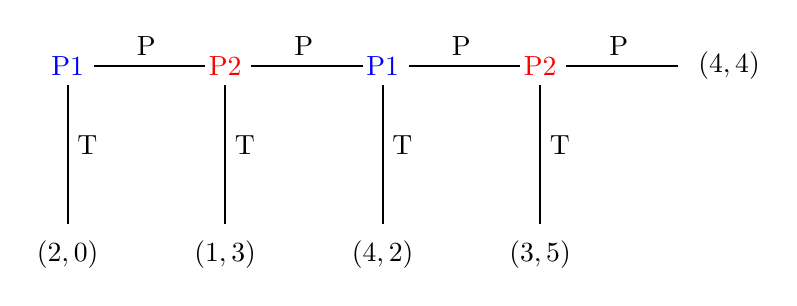
\begin{tikzpicture}
            \node (A) at (0,0) [blue] {P1};
            \node (B) at ($(A) + (2,0) $) [red] {P2};
            \node (C) at ($(B) + (2,0) $) [blue] {P1};
            \node (D) at ($(C) + (2,0) $) [red] {P2};

            \foreach \n in {A, B, C, D}
                {
                    \draw [thick] (\n) -- ($(\n) + (0,-2)$);
                    \draw [thick] (\n) -- ($(\n) + (1.75,0)$);
                    \node at ($(\n) + (1,.25)$) {P};
                    \node at ($(\n) + (.25,-1)$) {T};
                }

                \node at ($(A) + (0,-2.4)$) {$(2,0)$};
                \node at ($(B) + (0,-2.4)$) {$(1,3)$};
                \node at ($(C) + (0,-2.4)$) {$(4,2)$};
                \node at ($(D) + (0,-2.4)$) {$(3,5)$};
                \node at ($(D) + (2.4,0)$) {$(4,4)$};

        \end{tikzpicture}
    \end{center}
}

\frame{
    \begin{center}
        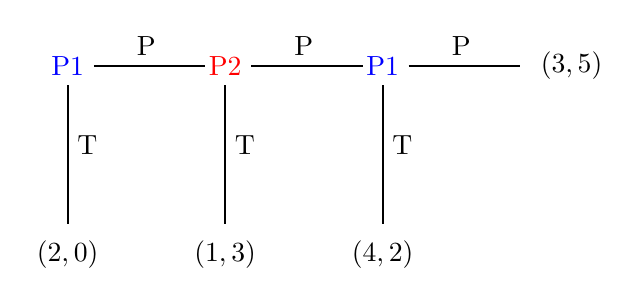
\begin{tikzpicture}
            \node (A) at (0,0) [blue] {P1};
            \node (B) at ($(A) + (2,0) $) [red] {P2};
            \node (C) at ($(B) + (2,0) $) [blue] {P1};

            \foreach \n in {A, B, C}
                {
                    \draw [thick] (\n) -- ($(\n) + (0,-2)$);
                    \draw [thick] (\n) -- ($(\n) + (1.75,0)$);
                    \node at ($(\n) + (1,.25)$) {P};
                    \node at ($(\n) + (.25,-1)$) {T};
                }

                \node at ($(A) + (0,-2.4)$) {$(2,0)$};
                \node at ($(B) + (0,-2.4)$) {$(1,3)$};
                \node at ($(C) + (0,-2.4)$) {$(4,2)$};
                \node at ($(C) + (2.4,0)$) {$(3,5)$};

        \end{tikzpicture}
    \end{center}
}

\frame{
    \begin{center}
        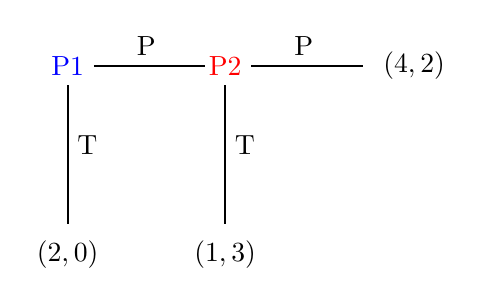
\begin{tikzpicture}
            \node (A) at (0,0) [blue] {P1};
            \node (B) at ($(A) + (2,0) $) [red] {P2};

            \foreach \n in {A, B}
                {
                    \draw [thick] (\n) -- ($(\n) + (0,-2)$);
                    \draw [thick] (\n) -- ($(\n) + (1.75,0)$);
                    \node at ($(\n) + (1,.25)$) {P};
                    \node at ($(\n) + (.25,-1)$) {T};
                }

                \node at ($(A) + (0,-2.4)$) {$(2,0)$};
                \node at ($(B) + (0,-2.4)$) {$(1,3)$};
                \node at ($(B) + (2.4,0)$) {$(4,2)$};

        \end{tikzpicture}
    \end{center}
}

\frame{
    \begin{center}
        \begin{tikzpicture}
            \node (A) at (0,0) [blue] {P1};

            \foreach \n in {A}
                {
                    \draw [thick] (\n) -- ($(\n) + (0,-2)$);
                    \draw [thick] (\n) -- ($(\n) + (1.75,0)$);
                    \node at ($(\n) + (1,.25)$) {P};
                    \node at ($(\n) + (.25,-1)$) {T};
                }

                \node at ($(A) + (0,-2.4)$) {$(2,0)$};
                \node at ($(A) + (2.4,0)$) {$(1,3)$};

        \end{tikzpicture}\\
        \onslide<2>{
        Nash equilibrium: \((\text{TT},\text{TT})\).
    }
    \end{center}
}

\frame{
    \begin{center}
        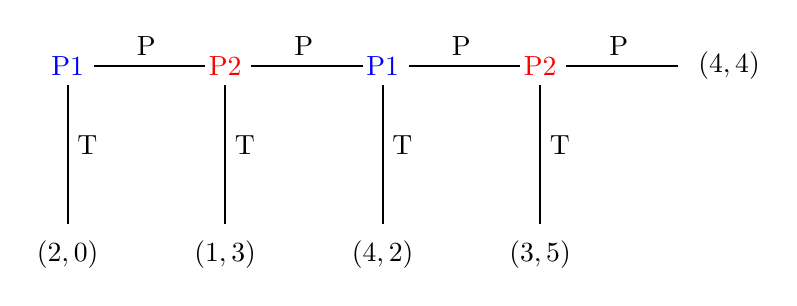
\begin{tikzpicture}
            \node (A) at (0,0) [blue] {P1};
            \node (B) at ($(A) + (2,0) $) [red] {P2};
            \node (C) at ($(B) + (2,0) $) [blue] {P1};
            \node (D) at ($(C) + (2,0) $) [red] {P2};

            \foreach \n in {A, B, C, D}
                {
                    \draw [thick] (\n) -- ($(\n) + (0,-2)$);
                    \draw [thick] (\n) -- ($(\n) + (1.75,0)$);
                    \node at ($(\n) + (1,.25)$) {P};
                    \node at ($(\n) + (.25,-1)$) {T};
                }

                \node at ($(A) + (0,-2.4)$) {$(2,0)$};
                \node at ($(B) + (0,-2.4)$) {$(1,3)$};
                \node at ($(C) + (0,-2.4)$) {$(4,2)$};
                \node at ($(D) + (0,-2.4)$) {$(3,5)$};
                \node at ($(D) + (2.4,0)$) {$(4,4)$};

        \end{tikzpicture}\\
        \only<1>{
        Nash equilibrium: \((\text{TT},\text{TT})\).
    }
        \only<2>{
            Nash equilibrium: \(\{(\text{TT},\text{TT}),(\text{TP},\text{TT}),(\text{TT},\text{TP}),(\text{TP},\text{TP})\}\).
        }
    \end{center}
}

\frame{
    \begin{center}
        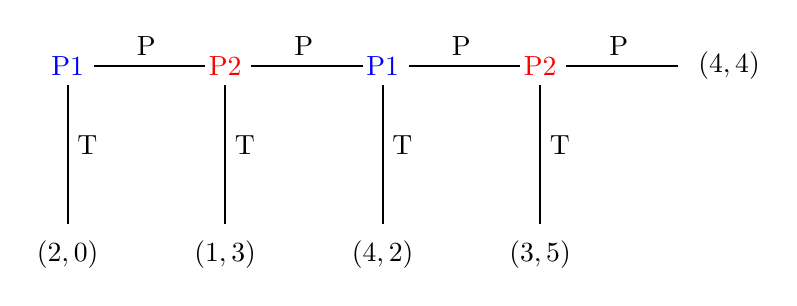
\begin{tikzpicture}
            \node (A) at (0,0) [blue] {P1};
            \node (B) at ($(A) + (2,0) $) [red] {P2};
            \node (C) at ($(B) + (2,0) $) [blue] {P1};
            \node (D) at ($(C) + (2,0) $) [red] {P2};

            \foreach \n in {A, B, C, D}
                {
                    \draw [thick] (\n) -- ($(\n) + (0,-2)$);
                    \draw [thick] (\n) -- ($(\n) + (1.75,0)$);
                    \node at ($(\n) + (1,.25)$) {P};
                    \node at ($(\n) + (.25,-1)$) {T};
                }

                \node at ($(A) + (0,-2.4)$) {$(2,0)$};
                \node at ($(B) + (0,-2.4)$) {$(1,3)$};
                \node at ($(C) + (0,-2.4)$) {$(4,2)$};
                \node at ($(D) + (0,-2.4)$) {$(3,5)$};
                \node at ($(D) + (2.4,0)$) {$(4,4)$};

        \end{tikzpicture}
        \pause
        $$\Leftrightarrow$$
        $S_1=S_2=\{PP,PT,TP,TT\}$
        \only<3>{
        $$
        \begin{pmatrix}
            (4,4) & (3,5) & (1,3) & (1,3)\\
            (4,2) & (4,2) & (1,3) & (1,3)\\
            (2,0) & (2,0) & (2,0) & (2,0)\\
            (2,0) & (2,0) & (2,0) & (2,0)\\
        \end{pmatrix}
        $$
    }
        \only<4,5>{
        $$
        \begin{pmatrix}
            (\underline{4},4) & (3,5) & (1,3) & (1,3)\\
            (\underline{4},2) & (\underline{4},2) & (1,\underline{3}) & (1,\underline{3})\\
            (2,\underline{0}) & (2,\underline{0}) & (\underline{2},\underline{0}) & (\underline{2},\underline{0})\\
            (2,\underline{0}) & (2,\underline{0}) & (\underline{2},\underline{0}) & (\underline{2},\underline{0})\\
        \end{pmatrix}
        $$
    }
        \onslide<5>{
        Nash equilibrium: \(\{(\text{TT},\text{TT}),(\text{TP},\text{TT}),(\text{TT},\text{TP}),(\text{TP},\text{TP})\}\).
    }
    \end{center}
}

\frame{
    \begin{center}
        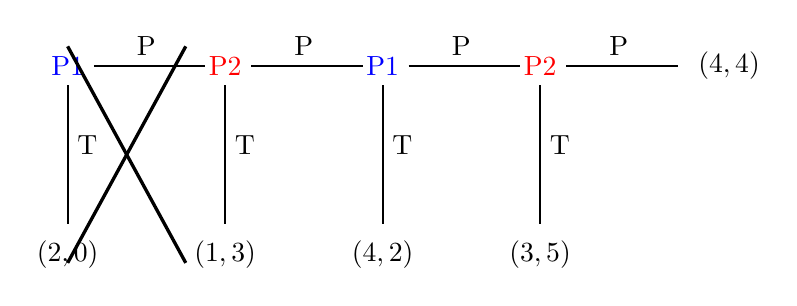
\begin{tikzpicture}
            \node (A) at (0,0) [blue] {P1};
            \node (B) at ($(A) + (2,0) $) [red] {P2};
            \node (C) at ($(B) + (2,0) $) [blue] {P1};
            \node (D) at ($(C) + (2,0) $) [red] {P2};

            \foreach \n in {A, B, C, D}
                {
                    \draw [thick] (\n) -- ($(\n) + (0,-2)$);
                    \draw [thick] (\n) -- ($(\n) + (1.75,0)$);
                    \node at ($(\n) + (1,.25)$) {P};
                    \node at ($(\n) + (.25,-1)$) {T};
                }

                \node at ($(A) + (0,-2.4)$) {$(2,0)$};
                \node at ($(B) + (0,-2.4)$) {$(1,3)$};
                \node at ($(C) + (0,-2.4)$) {$(4,2)$};
                \node at ($(D) + (0,-2.4)$) {$(3,5)$};
                \node at ($(D) + (2.4,0)$) {$(4,4)$};

                \draw [very thick] (0,.25) -- (1.5,-2.5);
                \draw [very thick] (1.5,0.25) -- (0,-2.5);

        \end{tikzpicture}
        \pause
        $$\Leftrightarrow$$
        $$S_1=\{\_P,\_T\}$$
        $$S_2=\{PP,PT,TP,TT\}$$
        \only<3>{
        $$
        \begin{pmatrix}
            (4,4) & (3,5) & (1,3) & (1,3)\\
            (4,2) & (4,2) & (1,3) & (1,3)\\
        \end{pmatrix}
        $$
    }
        \only<4-6>{
        $$
        \begin{pmatrix}
            (\underline{4},4) & (3,\underline{5}) & (\underline{1},3) & (\underline{1},3)\\
            (\underline{4},2) & (\underline{4},2) & (\underline{1},\underline{3}) & (\underline{1},\underline{3})\\
        \end{pmatrix}
        $$
    }
        \onslide<5-6>{
        Nash equilibrium: \(\{(\text{\_T},\text{TP}),(\text{\_T},\text{TT})\}\).
    }\\
        \onslide<6>{
            Original equilibrium: \(\{(\text{TT},\text{TT}),\cancel{(\text{TP},\text{TT})},(\text{TT},\text{TP}),\cancel{(\text{TP},\text{TP})}\}\).
    }
    \end{center}
}

\frame{
    \begin{center}
        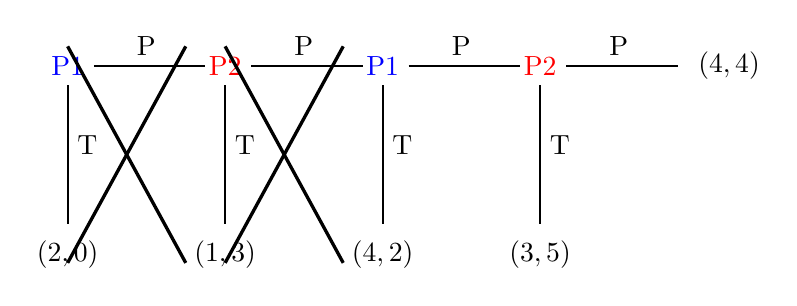
\begin{tikzpicture}
            \node (A) at (0,0) [blue] {P1};
            \node (B) at ($(A) + (2,0) $) [red] {P2};
            \node (C) at ($(B) + (2,0) $) [blue] {P1};
            \node (D) at ($(C) + (2,0) $) [red] {P2};

            \foreach \n in {A, B, C, D}
                {
                    \draw [thick] (\n) -- ($(\n) + (0,-2)$);
                    \draw [thick] (\n) -- ($(\n) + (1.75,0)$);
                    \node at ($(\n) + (1,.25)$) {P};
                    \node at ($(\n) + (.25,-1)$) {T};
                }

                \node at ($(A) + (0,-2.4)$) {$(2,0)$};
                \node at ($(B) + (0,-2.4)$) {$(1,3)$};
                \node at ($(C) + (0,-2.4)$) {$(4,2)$};
                \node at ($(D) + (0,-2.4)$) {$(3,5)$};
                \node at ($(D) + (2.4,0)$) {$(4,4)$};

                \draw [very thick] (0,.25) -- (1.5,-2.5);
                \draw [very thick] (1.5,0.25) -- (0,-2.5);
                \draw [very thick] (2,.25) -- (3.5,-2.5);
                \draw [very thick] (3.5,0.25) -- (2,-2.5);

        \end{tikzpicture}
        \pause
        $$\Leftrightarrow$$
        $$S_1=S_2=\{\_P,\_T\}$$
        \only<3>{
        $$
        \begin{pmatrix}
            (4,4) & (3,5)\\
            (4,2) & (4,2)\\
        \end{pmatrix}
        $$
    }
        \only<4-6>{
        $$
        \begin{pmatrix}
            (\underline{4},4) & (3,\underline{5})\\
            (\underline{4},\underline{2}) & (\underline{4},\underline{2})\\
        \end{pmatrix}
        $$
    }
        \onslide<5-6>{
        Nash equilibrium: \(\{(\text{\_T},\text{\_P}),(\text{\_T},\text{\_T})\}\).
    }\\
        \onslide<6>{
            Original equilibrium: \(\{(\text{TT},\text{TT}),\cancel{(\text{TP},\text{TT})},(\text{TT},\text{TP}),\cancel{(\text{TP},\text{TP})}\}\).
    }
    \end{center}
}

\frame{
    \begin{center}
        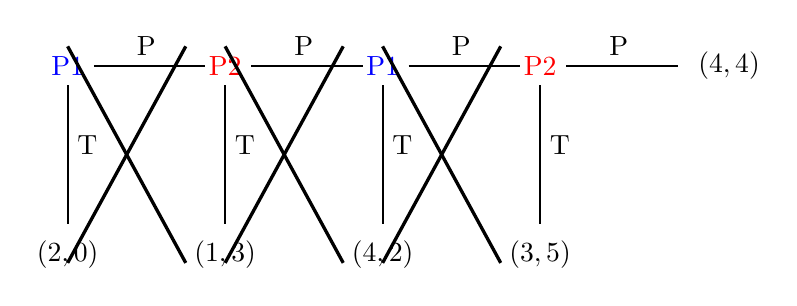
\begin{tikzpicture}
            \node (A) at (0,0) [blue] {P1};
            \node (B) at ($(A) + (2,0) $) [red] {P2};
            \node (C) at ($(B) + (2,0) $) [blue] {P1};
            \node (D) at ($(C) + (2,0) $) [red] {P2};

            \foreach \n in {A, B, C, D}
                {
                    \draw [thick] (\n) -- ($(\n) + (0,-2)$);
                    \draw [thick] (\n) -- ($(\n) + (1.75,0)$);
                    \node at ($(\n) + (1,.25)$) {P};
                    \node at ($(\n) + (.25,-1)$) {T};
                }

                \node at ($(A) + (0,-2.4)$) {$(2,0)$};
                \node at ($(B) + (0,-2.4)$) {$(1,3)$};
                \node at ($(C) + (0,-2.4)$) {$(4,2)$};
                \node at ($(D) + (0,-2.4)$) {$(3,5)$};
                \node at ($(D) + (2.4,0)$) {$(4,4)$};

                \draw [very thick] (0,.25) -- (1.5,-2.5);
                \draw [very thick] (1.5,0.25) -- (0,-2.5);
                \draw [very thick] (2,.25) -- (3.5,-2.5);
                \draw [very thick] (3.5,0.25) -- (2,-2.5);
                \draw [very thick] (4,.25) -- (5.5,-2.5);
                \draw [very thick] (5.5,0.25) -- (4,-2.5);

        \end{tikzpicture}
        \pause
        $$\Leftrightarrow$$
        $$S_2=\{\_P,\_T\}$$
        \only<3>{
        $$
        \begin{pmatrix}
            (4,4) & (3,5)\\
        \end{pmatrix}
        $$
    }
        \only<4-6>{
        $$
        \begin{pmatrix}
            (4,4) & (3,\underline{5})\\
        \end{pmatrix}
        $$
    }
        \onslide<5-6>{
            Nash equilibrium: \(\{\text{\_T}\}\).
    }\\
        \onslide<6>{
            Original equilibrium: \(\{(\text{TT},\text{TT}),\cancel{(\text{TP},\text{TT})},\cancel{(\text{TT},\text{TP})},\cancel{(\text{TP},\text{TP})}\}\).
    }
    \end{center}
}
\end{document}
